%% LyX 2.3.6.1 created this file.  For more info, see http://www.lyx.org/.
%% Do not edit unless you really know what you are doing.
\documentclass[american]{report}
\usepackage[T1]{fontenc}
\usepackage[latin9]{inputenc}
\setcounter{secnumdepth}{3}
\setcounter{tocdepth}{3}
\usepackage{amsbsy}
\usepackage{graphicx}
\PassOptionsToPackage{normalem}{ulem}
\usepackage{ulem}

\makeatletter
%%%%%%%%%%%%%%%%%%%%%%%%%%%%%% Textclass specific LaTeX commands.
\newenvironment{lyxlist}[1]
	{\begin{list}{}
		{\settowidth{\labelwidth}{#1}
		 \setlength{\leftmargin}{\labelwidth}
		 \addtolength{\leftmargin}{\labelsep}
		 \renewcommand{\makelabel}[1]{##1\hfil}}}
	{\end{list}}

%%%%%%%%%%%%%%%%%%%%%%%%%%%%%% User specified LaTeX commands.
\usepackage{culmus}

\makeatother

\usepackage{babel}
\begin{document}

\chapter*{Theorterical Part:}

%\section*{Question 1:}
%
%\uline{Pros:}
%\begin{itemize}
%\item Very easy to calculate (computational good)
%\item It's good indication for the first part of the game- when you have
%to stop the opponent from completing a mill.
%\end{itemize}
%\uline{Cons:}
%\begin{itemize}
%\item This heuristic doesn\textquoteright t give a very good indication
%of the position evaluation:
%\begin{itemize}
%\item It's don't take into account the number of soldiers each player has.
%\item It's don't take into account the fact that the mobility is important
%in this game- a player which can't perform a move is losing
%\end{itemize}
%\item \textbf{Jacob TODO:copy here an examples and explain}
%\end{itemize}

\section*{Question 2}

We will define the next heuristic:

\[
h(s)=Eval(White)-Eval(Black)
\]

if $h(s)>0$ white is better, else black is better.

We will define the evaluation fuction of each player by a weigheted
sum:

\[
Eval(Player)=\sum_{i=1}c_{i}R_{i}
\]

R1= Number of closed mills: +1 If a mill was closed in the last move
by the player

R2= Number of mills

R3 = Number of blocked opponent pieces- pieces which don\textquoteright t
have an empty adjacent point

R4= Number of pieces

R5= Number of 2-piece configuration (2 mans and one empty in a line)

R6= Number of 3-piece configurations (A 3-piece configuration is one
to which a piece can be added in which one of two ways to close a
mills)

\textbf{Jacob TODO: rewriting the next paragraph (currently it's just
copied from web)}

R7= Double morris: Difference between number of yours and yours opponent\textquoteright s
double morrises (A double morris is one in which two morrises share
a common piece)

R8=Winning configuration: 1 if the state is winning for the player,
-1 if losing, 0 otherwise For the particular contest settings (elimination
with the player having more pieces winning if neither side could force
a win so there was a strong aversion to sacrificing material) and
bot settings (depth limited to 8 and branching factor limited to 20;
at each step, top 20 moves sorted by the evaluation function were
selected), I found the following feature combinations to work well
(\textquoteleft (1)\textquoteright{} represents the first feature:
Closed Morris and so on) \\

The motivation of using that heuristic is from a peper : ``Nine Men\textquoteright s
Morris: Evaluation Functions'' by: Simona-Alexandra PETCU, Stefan
HOLBAN

\textbf{Jacob TODO: explain about coeeficients. Explain that for diffrent
part of the game we use diffrent} $c_{i}$

\textbf{In practice we don't have to use that complex heuristic, we
can choose only 4 parameters between the 8 described above....}

%\section*{Question 3}
%\begin{description}
%\item [{a)}]~
%\end{description}
%The advantage of Alpha-beta pruning algorithm is that it \textbf{decrease
%the number of nodes that evaluated} by an Minimax algorithm, although
%the selected move will be the same as in the regular minimax algorithm.By
%using the pruning, branches of the search tree can be eliminated,
%and \textbf{a deeper search can be performed}.\\
%This advantage achieved by avoiding seaching subtrees of moves which
%won't be selected.\\
%Algorithm Explanation\footnote{Based on: ``Alpha-Beta Pruning: Algorithm and Analysis'' by Tsan-sheng
%Hsu}:
%
%for simplicity assuming a max node (Alpha cut off):
%\begin{description}
%\item [{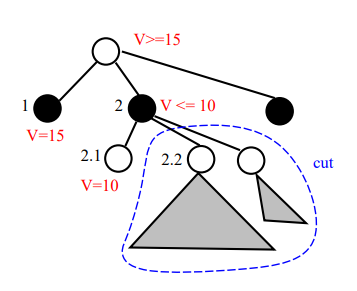
\includegraphics{Pics/3_a_1}}]~
%\end{description}
%\begin{itemize}
%\item Assume you have finished exploring the branch at 1 and obtained the
%best value from it as $bound$.
%\item You now search the branch at 2 by first searching the branch at 2.1.
%\item Assume branch at 2.1 returns a value that is $\le bound$.
%\item Then no need to evaluate the branch at 2.2 and all later branches
%of 2, if any, at all.
%\item The best possible value for the branch at 2 must be $\le bound$.
%\item Hence we should take value returned from the branch at 1 as the best
%possible solution.
%\end{itemize}
%\begin{description}
%\item [{b)}] (from Lecture No.5 slide 35) \\
%Optimal pruning happens when the extreme (min./max) value of every
%node is found first: \\
%In max nodes the highest minimax value is found in the first child\\
%In min nodes the lowest minimax value is found in the first child
%\item [{c)}]~
%\end{description}
%No leaf will be pruned by alpha-beta :
%\begin{description}
%\item [{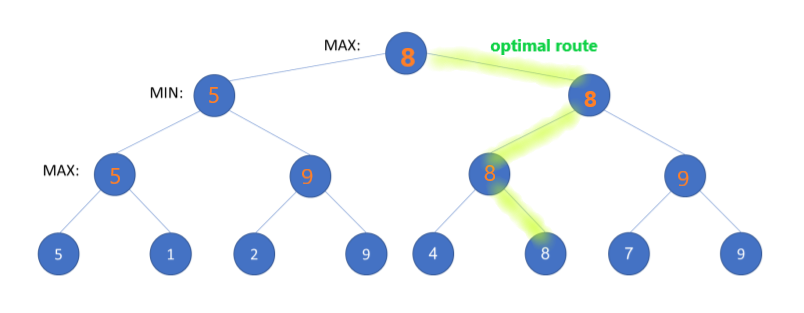
\includegraphics[scale=0.6]{report_Images/image3_0}}] \\
%\end{description}
%

\section*{Question 4}

Alpha beta pruning with some heuristic gave us exactly the same result
(move) as minimax (with less calculations)

minimax algorithm with limited resources is as good as it's heuristic....

Minimax strategy is inefficient, since it discourages taking any risks,
no matter how high the reward may be- It's takes the safe routes.\\


\section*{Question 5}
\begin{lyxlist}{00.00.0000}
\item [{a)}]~
\item [{b)}]~
\item [{c)}]~
\end{lyxlist}
TODO\\


%\section*{Question 6}
%
%A student implemts an alpha-beta algorithm and in a game against the
%software she noticed that the computer didn't take a winning move
%(in the next step) and chose another step.
%
%a. such situation possible because the heuristic mislead us-the wining
%move had lower heuristic value than the move actually performed. Probably,
%the used heuristic doesn't evaluate if the position end of the game.
%
%b. The Change that we can perform is that if the alpha-beta algorithm
%gets a state that is winning for the Agent than it return that move.
%
%In the picture below we can see the regular alpha-beta.
%
%The change on the algorithm proposed:
%
%G=G(state,agent) - get's also the agent (True for maximizing agent
%)
%
%G(state,agent) has to return an tuple (\{T,F\},\{T,F\}) - the first
%boolean value is True if the state is endgame and the second is True
%if it's the end of the game and Agent won.
%
%If G(state) is (True,True) need to return $-\infty$ or $\infty$
%depenting if that a min agent or max agent respectively.
%
%And the same for (True,False) return $\pm\infty$ depends on the agent
%type.
%
%That way we can guarantee that the winning move is always will be
%returned.
%
%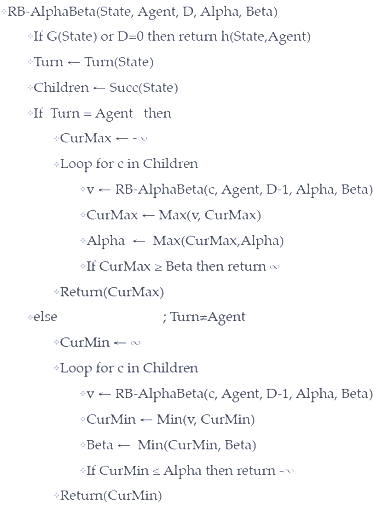
\includegraphics{Pics/6_b}

\section*{Question 7}

%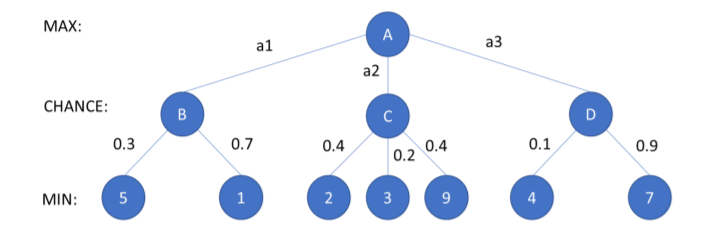
\includegraphics[scale=0.6]{report_Images/7_0}\\
%
%\begin{lyxlist}{00.00.0000}
%\item [{a)}] The expectimax of a chance node is calculated by a weighted
%sum of the utility and the probability to get it.\\
%$U(B)=0.3\cdot5+0.7\cdot1=2.2$\\
%$U(C)=0.4\cdot2+0.2\cdot3+0.4\cdot9=5$\\
%$U(D)=0.1\cdot4+0.9\cdot7=6.7$
%\item [{b)}] The max operator takes the path with the best value at the
%chance node:\\
%$U(A)=U(argmax(U(i))=U(D)=6.7$\\
% \textbf{Thus action D}
%\item [{c)}] NO we can't perform an alpha-beta pruning in an expectimax
%nodes because we can't calculate the expectimax value until we haven't
%exposed all the nodes.\\
%We can perform a pruning if we got a higher and a lower bound of the
%leaves.\\
%The regular Expectimax is calculated by $Expectimax(state,action)=\sum_{i\in succ(state,action)}p_{i}u_{i}$
%where p,u are the probability and utility.\\
%If we got a upper and lower bound of the utility $(u_{min},u_{max})$
%we can predict the bounds of Expectimax node after revealing one possible
%successor:
%\[
%Expectimax(state,action)\in[p_{1}\cdot u_{1}+(1-p_{1})\cdot u_{min},p_{1}\cdot u_{1}+(1-p_{1})\cdot u_{max}]
%\]
%\\
%But if not given an upper and lower bound, we can't prune for example:
%\item [{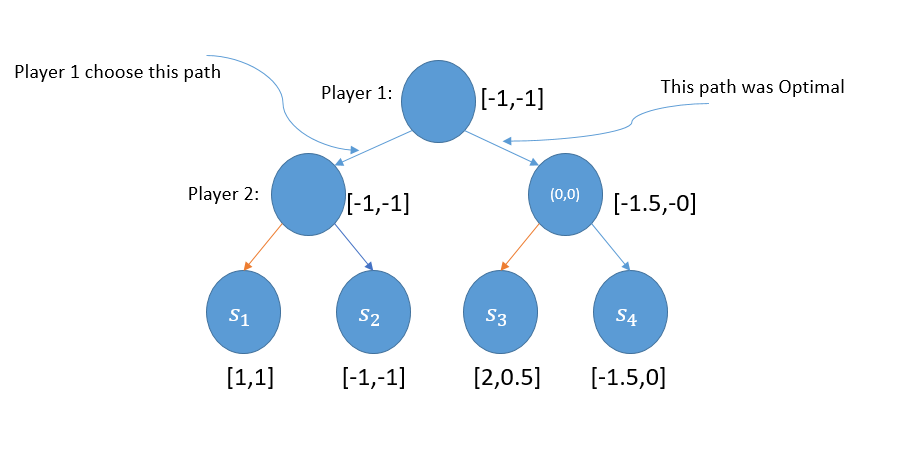
\includegraphics{Pics/7_c}}]~
%\end{lyxlist}
%Assume the first action was been evaluated and the Expectimin returned
%2.2 . Now we need to evaluate the next action (a2).
%
%The first successor looks promessing with high probability and value
%we already get 2.4 on our a2 chance node and seems that we don't need
%to check the next leaves...
%
%However what if the value in D \textbackslash{} is negative and equals
%to -2? Than the result of the Expectimin operator on the second action
%equals 2 (smaller then a1 action)
%
%That's why naive approach won't work.
%
%(if we had some bound on the leaves e.g. positive value utility, we
%could say in the above example that after checking one leaf at the
%a2 action we coul'd guarantee that action a1 is better).

\section*{Question 8}

TODO

\section*{Question 9}

%\textbf{$\boldsymbol{d_{2}=\mathcal{O}(2\cdot d_{1}})$ }
%
%The time complexity of minimax is $O(b^{d})$ i.e. function of the
%number ot leaves in the deepest searching layer.
%
%If we get the rival\_move we don't need to expand the whole opponent
%possible moves,just need to run this procedure.
%
%Thus the tree size multiply by $b$ every two layers of actions (our
%node increase it by factor of $b$ and opponent move leaves it the
%same size).
%
%$O(b^{d_{1}})=O(b^{d_{2}/2})$ i.e. $d_{2}=2\cdot d_{1}$ (This is
%by asymptotic analysis)
%
%b.
%
%Q:Given state s what is the ratio between the value of the minimax
%with use of the procedure and the value of the minimax without of
%the procedure when both limitted to depth $d$ ?
%
%The minimax value is the highest value that the player can be sure
%to get without knowing the actions of the opponent-It is the lowest
%value the rival can force the player to receive.
%
%$v_{i}=max(min(v_{i}))$
%
%Minimax strategy assumes a perfect opponent,i.e. choosing the worst
%scenerio for our agent , but the rival don't neccesserely choose the
%action with the lowest utility (not the min)\\
%\textbf{Thus minimax value without using rival\_move procedure < minimax
%with using rival\_move procedure.}

\section*{Question 10}

Given: maximiziation problem with search space of size $10^{12}$

Solving with random-restart hill climbing.

Runing the algorithm $10^{3}$ times

a.

The student isn't necceseserly right to report that the optimum is
at 5.8.

The reason is that he has been using a randomized algorithm and $10^{3}$
runs are low with respect to the state space size $10^{12}$ , thus
\textbf{his result isn't statistical significant}.

b. If we had to varify the student's result we would use a \textbf{simulated
annealing algorithm}.

The problem of SAHC algorithms is that they try to maximize the state
and never makes ``down-hill moves'' toward states with lower value.

In contrast, \textbf{simulated annealing allows moving to states with
lower value}.

c.

Add image and few word of explanation.

\chapter*{Wet Part:}
\end{document}
